\section{Introduction}
Databases are susceptible to various forms of corruption, or \emph{dirtiness}, such as missing, incorrect, or inconsistent values.
Numerous industrial surveys have shown that dirty data are prevalent \cite{Gartner}, and there is now a growing industry around cleaning data at scale \cite{fortunearticle}.
Recent research and commercial interest is driven by increasing analytics from inherently error-prone processes such as extracting structured data from websites and synthesizing data from noisy sensors.
New methodologies for scalable and reliable analysis in the presence of errors are required. 

Data analysis pipelines are also growing in complexity.
The endpoint of these pipelines can be any number of ``data products", such as recommender systems, spam detectors, and forecasting models, all of which can be very sensitive to data quality \cite{xiaofeature}.
Increasingly, analytics stacks are moving beyond traditional SQL analytics and natively supporting Machine Learning (e.g. Berkeley Data Analytics Stack \cite{bdas}, Hadoop, Stratosphere \cite{alexandrov2014stratosphere}).
Predictions made by Machine Learning models can be significantly affected by systematic dirtiness i.e., corruption that is correlated with the data.
Consider a music recommender system, we may find that due to a software bug all users from Europe have an incorrect age attribute defaulted to ``18-24".
A recommendation model trained on this data may spuriously ``learn" a correlation relationship between the ``18-24" age group and music liked by European users.
While there is an extensive literature on robust Machine Learning, this work largely focuses on resilience to atypical outliers (i.e., age of ``1000") and not systematically corrupted data.

Since new analytics frameworks encapsulate the entire data processing pipeline from raw data to features to model training, there is an opportunity to address this problem from an end-to-end data management perspective.  
The database community's response to systematic corruption is data cleaning, which is an extensively studied field (see Rahm and Do \cite{rahm2000data} for a survey).
Cleaning works by repairing (or approximately repairing) the corruption in the base data.
However, data cleaning can be a very time consuming process.
Programming data transformations to fix all problems manifest in the data requires substantial developer effort \cite{kandel2012}.
As errors increase in complexity, scripted transformations and automated rules may not suffice. 
Works such as Corleone\cite{gokhale2014corleone} and CrowdFill\cite{park2014crowdfill} address this problem by using crowdsourcing.
While more it is more accurate, even moderately sized datasets are very challenging to clean with the crowd.

An emerging solution to the growing costs of data cleaning is sampling as proposed in the SampleClean work\cite{wang1999sample}. The analyst cleans a small sample of $k \ll N$ records and can estimate the results of aggregate queries based on cleaning this sample.
Adjusting the sample size $k$ provides a flexible tradeoff between cleaning cost and query result accuracy for aggregate queries.
The case for sampling in data cleaning is analogous to arguments for Approximate Query Processing (AQP) \cite{DBLP:conf/eurosys/AgarwalMPMMS13}, where a timely approximate answer is more desirable than an exact slow answer. 

\begin{figure}[t]
\centering
 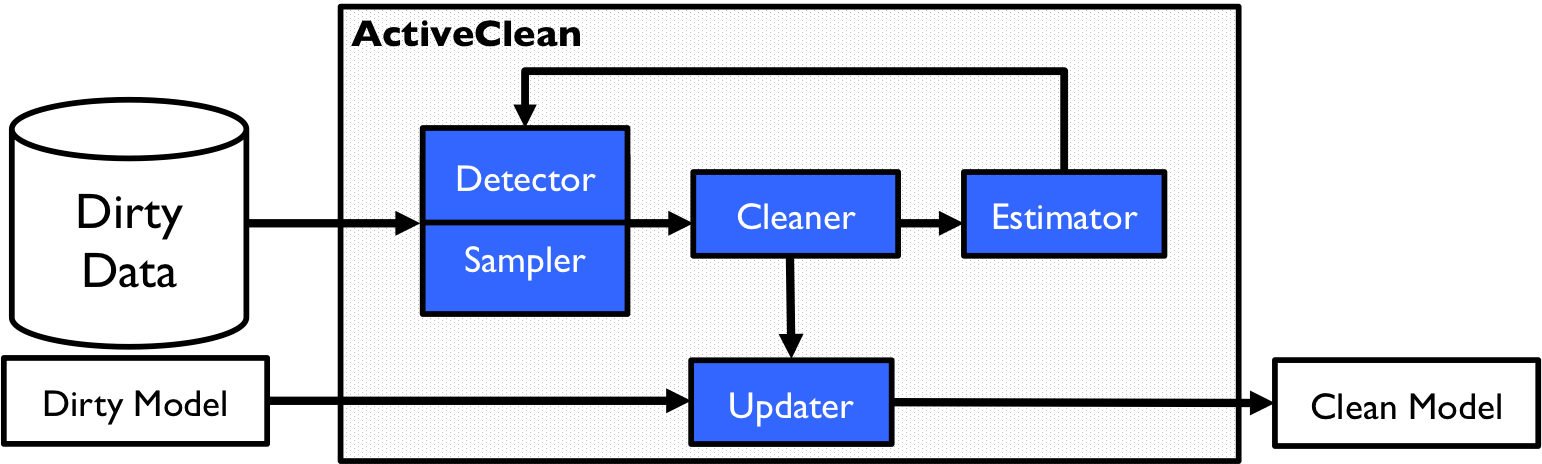
\includegraphics[width=\columnwidth]{figs/arch.png}
 \caption{\sysfull presents an architecture where data cleaning is integrated with model training. The user specifies a data repair method, and we provide a framework for sampling, model update, and feedback through estimation. \label{sys-arch}}\vspace{-2em}
\end{figure}

Unfortunately, a naive application of sampling will not work well for the high-dimensional models learned in Machine Learning.
These applications are far more sensitive to sample size (training data) than aggregate queries.
Machine Learning applications can require a large amount of training data to learn correlations between possibly hundreds of features and labels.
A small sample of clean data may not be able to support a viable Machine Learning model.
The predictions from this model may be inaccurate and the problems introduced by the small sample size may dominate any gains from data cleaning. 

In this paper, we propose \sys, an anytime framework for training Machine Learning models with budgeted data cleaning (Figure \ref{sys-arch}) that iteratively corrects a dirty model rather than retraining it on a sample of clean data.
\sys is initialized with a dirty model and users specify a repair method.
Our system will provide a framework to return an accurate model given a repair budget.
\sys selects a sample of data, applies the repairs, then updates the model.
After model update, the repairs are fed back to adaptively select the next sample of data.
We can optionally integrate user specified dirty data detection rules (such as constraints) into the framework to further narrow our sampling.
\sys supports a broad class of models, called convex-loss models, which includes linear regression, logistic regression, generalized linear models, and support vector machines.

\sys presents a novel framework that tightly integrates data cleaning with model training.
As a result, there are numerous new opportunities for optimization.
We can ``push down" the model training to the data cleaning and select data to clean that are most valuable to the model.
We can also ``push up" the data cleaning to the model training by intelligently batching together model updates from already cleaned data.
In summary, our contributions are
\begin{itemize}[noitemsep]
\item We propose \sysfull which given dirty data, a model, a data cleaning procedure, and a budget, we can return a highly accurate model for a fraction of the cleaning cost.
\item \sys proposes a novel framework that iteratively corrects a model based on small batches of clean data.
\item \sys relies on two key optimizations, guided error sampling and error partitioning, that result in substantial empirical gains in accuracy in comparison to alternative approaches such as Active Learning.
\item We evaluate \sysfull on real and synthetic datasets to show that non-uniform sampling achieves improved performance in comparison to uniform sampling, and Active Learning.
\end{itemize}






